\section{Einleitung}

\subsection{Arbeitsweise während der Implementierungsphase}
\begin{frame}
\frametitle{Die Arbeitsweise während der Implementierungsphase}

\begin{itemize}
	\item<+-> Ausnutzung der Verfügbarkeit hilfreicher Werkzeuge wie Bug-Tracker, Code-Review, Continuous-Integration mit automatischen Tests und statischer Analyse
	\item<+-> AST-Attrappenerstellung für Testprogramme
	\item<+-> Parallele Komponentenentwicklung
	\item<+-> Regelmäßige Treffen
\end{itemize}
\end{frame}

\subsection{Zeitlicher Ablauf}
\begin{frame}
\frametitle{Zeitlicher Ablauf}

\begin{figure}
	\vspace{-0.15cm}
	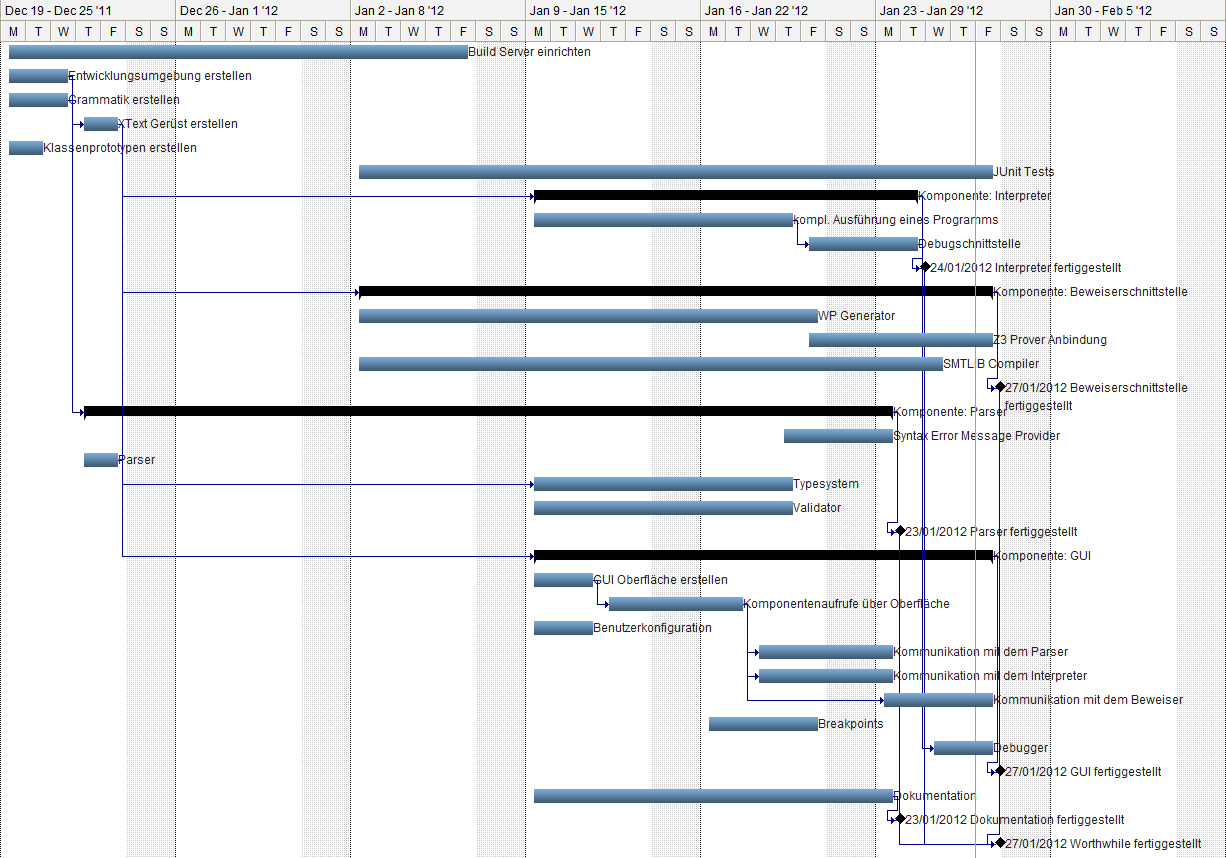
\includegraphics[height=0.95\textheight]{../bericht/images/gantt_implementierung_diag.png}
\end{figure}
\end{frame}
